%%
%
% ARQUIVO: cap-02.tex
%
% VERSÃO: 1.0
% DATA: Maio de 2017
% AUTOR: Carla Cosenza, Matheus Mello, Rebeca Reis
% 
%  Arquivo tex de exemplo de capítulo do documento de Projeto de Fim de Curso.
%
% ---
% DETALHES
%  a. todo capítulo deve começar com \chapter{•}
%  b. usar comando \noindent logo após \chapter{•}
%  c. citações para referências podem ser
%       i. \citet{•} para citações diretas (p. ex. 'Segundo Autor (2015)...'
%       ii. \citep{•} para citações indiretas (p. ex. '... (AUTOR, 2015)...'
%  d. notas de rodapé devem usar dois comandos
%       i. \footnotemark para indicar a marca da nota no texto
%       ii. \footnotetext{•}, na sequência, para indicar o texto da nota de rodapé
%  e. figuras devem seguir o exemplo
%       i. devem ficar no diretório /img e devem ser no formato EPS
%  f. tabelas devem seguir o exemplo
%  g. figuras e tabelas podem ser colocadas em orientação landscape
%       i. figuras: usar \begin{sidewaysfigure} ... \end{sidewaysfigure}
%                   em vez de \begin{figure} ... \end{figure}
%       ii. tabelas: usar \begin{sidewaystable} ... \end{sidewaystable}
%                    em vez de \begin{table} ... \end{table}
%  h. toda figura e tabela deve ser referenciada ao longo do texto com \ref{•}
% ---
%%

\chapter{Atividades Realizadas}
\noindent
\section{Estudos premilinares}

Antes de iniciar o projeto final, eu havia cursado a disciplina de compiladores. Durante esse mesmo semestre adquiri os conhecimentos de como construir um analisador léxico e um analisador sintático de forma satisfatória. No mesmo período, aprendi makefile e scripts shell. O ambiente de desenvolvimento utilizado é bastante inspirado no que eu usei para desenvolver o trabalho da disciplina de compiladores, em 2016.2.

Esses conhecimentos foram combinados com o conhecimento prévio que eu tinha com a linguagem brainfuck, para qual eu criei um produto comercial que vendi no ano de 2016. Contudo, apenas o conhecimento que tinha de brainfuck não foi suficiente para realizar o projeto e tive que procurar fontes especializadas para me ajudar a resolver o problema.

De antemão eu sabia que o proposto era possível. Eu havia, em minhas pesquisas, encontrado softwares que faziam coisas similares. Sabia, também, que os conhecimentos adquiridos na disciplina de compiladores e na disciplina de computabilidade, ambas em 2016.2, forneceriam uma fundação sólida para a construção dessa solução.

Foi criado um protótipo do projeto. Este contava com um analisador léxico e sintático, com uma representação em árvore de sintaxe abstrata e podia compilar programas simples para brainfuck. Programas como prints de constantes strings e operações de adição, subtração, multiplicação e divisão simples. Este protótipo foi criado no final de 2017.1

Além destes estudos, descobri projetos e analisei o github durante todo o projeto. Houve vários updates durante o desenvolvimento do projeto. A linguagem similar a Headache, Brain (feita em Rust) foi desenvolvida durante 2017. A página Brainfuck Algorithms foi atualizada com novos algoritmos, correções e distribuições durante o ano de 2017 e continua a ser atualizada. 

\section{Método}

O método seguido provém diretamente do que foi utilizado para desenvolver o compilador da disciplina de compiladores. Consiste em separar as funções de um compilador em divisões, regidas por suítes de teste, e ir compondo os testes a medida que o compilador vai avançando. Isso garante uma boa estabilidade a um programa que pode receber os mais diversos tipos de input. 

Foi seguido Desenvolvimento Orientado a Testes (Test Driven Development, TDD) durante todo o desenvolvimento. Por ser um compilador, os inputs e outputs são sempre conhecidos.

\begin{figure}[h]
	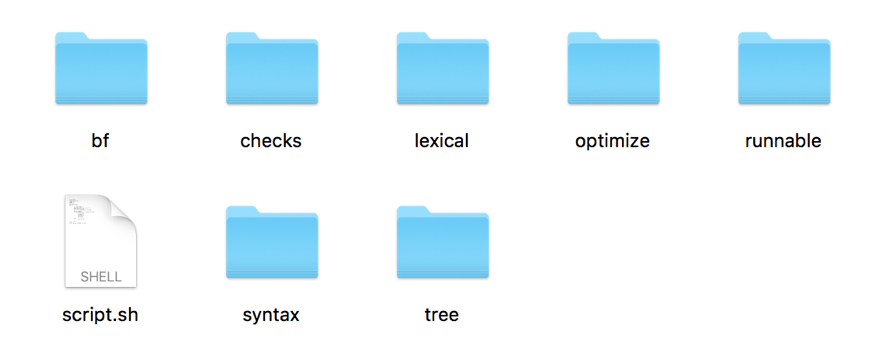
\includegraphics[]{TD/img/folders.png}
	\caption{Suítes de Teste do projeto}
	\label{folders}
\end{figure}

A features da linguagem eram implementadas de acordo com uma estimada ordem de dificuldade.
	
Boa parte do processo de desenvolvimento e do desafio do projeto foi a implementação dos algoritmos disponíveis na Brainfuck Algorithms e o fluxo de trabalho deste mesmo processo.
	
Abaixo há um exemplo de como o fluxo de trabalho de tradução dos algoritmos foi melhorando com o avanço do projeto.

Exemplo:

\begin{verbatim}
    /*   temp0[-]
            y[x+temp0+y-]
            temp0[y+temp0-]*/
\end{verbatim}

Esse é um algoritmo para adição dos valores de duas células (representadas por x e y). Ele é usado no hac para implementar adição entre duas variáveis de 1 byte (isto é, de uma célula). Os nomes presentes nesse algoritmo são, na verdade, abreviações de instruções para ir na célula nomeada de tal forma. (isto é, são abreviações de várias instruções > e <). Neste relatório, tal operação será chamada de goto. (Não confundir com a operação de fluxo de controle. O nome aqui é usado para uma operação referente a acesso a memória). 

É oportuno notar que todo uso da operação goto pode ser resolvido de forma estática. Como a operação goto é recorrente em todos os algoritmos públicos, foi criada uma função para ela:

\begin{verbatim}
    static void codeGoTo(int cellIndex){
        int units = unitsToMoveTo(cellIndex);
        char direction = '>';
        int count = 0;
        assert(currentCell + units == cellIndex)
        if(units < 0){
            direction = '<';
            units = -units;
        }
        currentCell += units;
        
        for( ; units > 0 ; units++){
            count++;
            fprintf(output, "%c" , direction);
        }
        currentCell = cellIndex;
    }
\end{verbatim}

Os algoritmos podem ser implementados por uma composição de impressão de strings com impressões da instrução goto. O algoritmo de adição acima, poderia ser implementado assim:

\begin{verbatim}
    static void incrementXbyY(int x, int y){
        printf("add %d to %d\n" , x, y);
        int temp0 = x - 1;
        codeGoTo(temp0); codeSt("[-]");
        codeGoTo(y); codeSt("["); codeSt(x); codeSt("+");
        codeGoTo(temp0); codeSt("+"); codeSt(y); codeSt("-]");
        codeGoTo(temp0); codeSt("["); codeSt(y); codeSt("+");
        codeGoTo(temp0); codeSt("-]");
    }
\end{verbatim}

Porém, esse estilo de implementação é muito ruim. É muito fácil cometer um erro: é preciso digitar muita coisa para pouco algoritmo. Há também uma grande dificuldade ler e verificar se há um goto para o endereço errado. Isso é particularmente notável quando os algoritmos ficam maiores:

\begin{verbatim}
    static void bfalgo(char* str, ...({
    \\based on http://www.gnu.org/software/libc/manual/html_node/Variadic-Example.html
        va_list ap;
        int i, j, sum;
        
        int count = 0;
        
        for(i = 0 ; str[i] ; i++){
            if(str[i] == '$' || str[i] == '@'){
                count++;
            }
        }
        printf("count %d\n" , count);
        va_start (ap, count);       /*Initialize the argument list.*/
        
        sum = 0;
        for(i = 0 ; str[i] ; i++){
            if(str[i] == '$'){
                int d = va_arg (ap, int);
                codeGoTo(d);
            } else if(str[i] == '@'){ //Not sure if I will use
                char* str = va_arg(ap, char*);
                codeStr(str);
            }
            else {
                fprintf(output, "%c" , str[i]);
            }
        }
        va_end (ap);                /* Clean up. */
    }
    
\end{verbatim}

\begin{verbatim}
    /*
    temp0[-]
    temp1[-]
    temp2[-]
    temp3[-]
    x[temp0+x-]
    temp0[
        y[temp1+temp2+y-]
        temp2[y+temp2-]
        temp1[
            temp2+
            temp0-[temp2[-]temp3+temp0-]
            temp3[temp0+temp1-]
            temp2[
                temp1-
                [x-temp1[-]]+
            temp2-]
        temp1-]
        x+
    temp0]
    */
\end{verbatim}

A solução para esse problema foi a implementação de uma função similar a printf para compor os algoritmos. Esta função recebe um número estaticamente variável de parâmetros (implementados com elipses em C). A função recebe a estrutura do algoritmo, em uma string, e, em seguida, os endereços das variáveis utilizadas para compor o algoritmo.

\begin{verbatim}
    /*   temp0[-]
            y[x+temp0+y-]
            temp0[y+temp0-]*/
            
    static void incrementXbyY(int x, int y){
        int temp0 = x-1;
        bfalgo("$[-] $[$+$+$-] $[$+$-]", temp0, y, x, temp0, y, temp0, y, temp0);
    }
\end{verbatim}

Pode-se observar que ela basicamente mantém o tamanho do texto original do algoritmo e é muito mais simples de ler e verificar se as variáveis estão nos locais corretos.

Embora a função bfalgo() facilitasse bastante o trabalho em relação ao método anterior, os temporários ainda tinham que ser colocados manualmente na chamada, e isso continuava sujeito aos erros do trabalho manual. Além disso a página Brainfuck Algorithms foi atualizada durante o desenvolvimento da Headache e era bastante trabalhoso adicionar manualmente novos algoritmos.

Para solucionar esse problema no fluxo de trabalho foi criado um utilitário chamado bfalgoConverter, que converte os algoritmos no formato da página Brainfuck Algorithms para chamadas da função bfalgo(). 

\begin{figure}[h]
	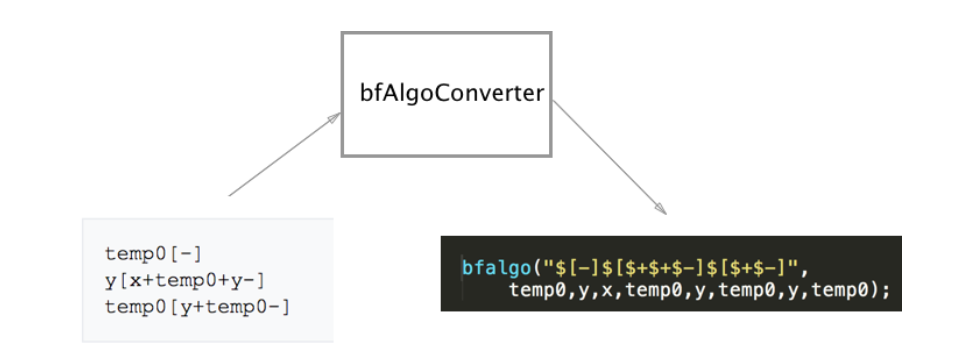
\includegraphics[]{TD/img/bfalgo.png}
	\caption{Esquema do bfalgoConveter}
	\label{folders}
\end{figure}

Ele foi implementado de uma maneira bastante hardcoded, porém, atende o seu propósito:

\begin{verbatim}
    char bigStr[1024*1024];     //1MB
    int tempList[999];
    int * tempListPtr = tempList;
    char* bigStrPtr = bigStr;
    while(fscanf(stdin, "%c" , &c) != EOF){
        if(!isBfChar(c)) {
            if(c == 't') {
                if(fscanf(stdin, "%c" , &c) != EOF){
                    if(c == 'e') {
                        if(fscanf(stdin, "%c" , &c) != EOF){
                            if(c == 'm') {
                                if(fscanf(stdin, "%c" , &c) != EOF){
                                    if(c == 'p'){
                                        if(fscanf(stdin, "%d" , &n) != EOF){
                                            *bigStrPtr = '$';
                                            bigStrPtr++;
                                            *tempListPtr = n;
                                            tempListPtr++;
                                            continue;
                                        }
                                    }
                                }
                            }
                        }
                    }
                }
            }
        }
        else{
            *bigStrPtr = c;
            if(c == 'x');
            ...
        }
    }
    
\end{verbatim} 

\section{Resultado}

Ao final temos, como produtos diretos deste estudo: o repositório de Headache no github; o compilador hac; o interpretador brainfuck bfi; o utilitário expansor de bitwidth expander; o utilitário de conversão dos algoritmos da Brainfuck Algorithms  bfalgoConverter, que converte códigos da webpage para as chamadas da função bfalgo(); a wiki da Headache no github e a EBNF de Headache no Anexo B.

\section{Cronograma}

O desenvolvimento de Headache foi bastante conturbado. Os cronogramas apresentados durante a proposta e durante o projeto final 1 divergem bastante de como foi efetivamente feito.  O desenvolvimento de Headache é público, devido a sua natureza open source, e pode ser verificado e acompanhado na página https://github.com/LucasMW/Headache/commits/master e https://github.com/LucasMW/Headache/graphs/contributors.

As principais diferenças entre os cronogramas se dá na ordem das tarefas e na concentração das tarefas em cada mês. Por exemplo:

A EBNF foi re-elaborada várias vezes; Prints dinâmicos de 8 bits foram concluídos antes de funções (embora prints de 8+ bits acabaram sendo concluídos, de fato, depois); A sintaxe e a AST foram atualizadas próximas ao fim do cronograma; etc.

Cronograma original:

\textbf{2017.1}

Abril:
\begin{itemize}
    \item Coletar /analisar bibliografia
    \item Elaboração da EBNF de Headache
\end{itemize}

Maio:
\begin{itemize}
    \item Descrição do modelo de memória de Headache 
    \item Início dos esboços de implementação
\end{itemize}

Junho:
\begin{itemize}
    \item Elaboração do relatório.
    \item Implementação do Analisador léxico
    \item Implementação do Analisador Sintático
    \item Implementação da Árvore Sintática Abstrata
\end{itemize}

\textbf{2017.2}

Julho:
\begin{itemize}
    \item Implementação de variáveis locais
    \item Completa implementação de expressões	
\end{itemize}

Agosto:
\begin{itemize}
    \item Revisão dos relatórios
    \item Implementação de variáveis globais
    \item Implementação completa da checagem de tipagem	
\end{itemize}

Setembro:
\begin{itemize}
    \item Implementação de funções e calls
    \item Implementação de Condições
    \item Implementação de if / else e while
\end{itemize}

Outubro:
\begin{itemize}
    \item Implementação do print dinâmico 
\end{itemize}

Novembro:
\begin{itemize}
    \item Revisão do código	
\end{itemize}

Extras:
\begin{itemize}
    \item Adicionar arrays tipados 
    \item Otimizar código gerado
\end{itemize}